% Created by tikzDevice version 0.12.6 on 2024-10-10 20:28:18
% !TEX encoding = UTF-8 Unicode
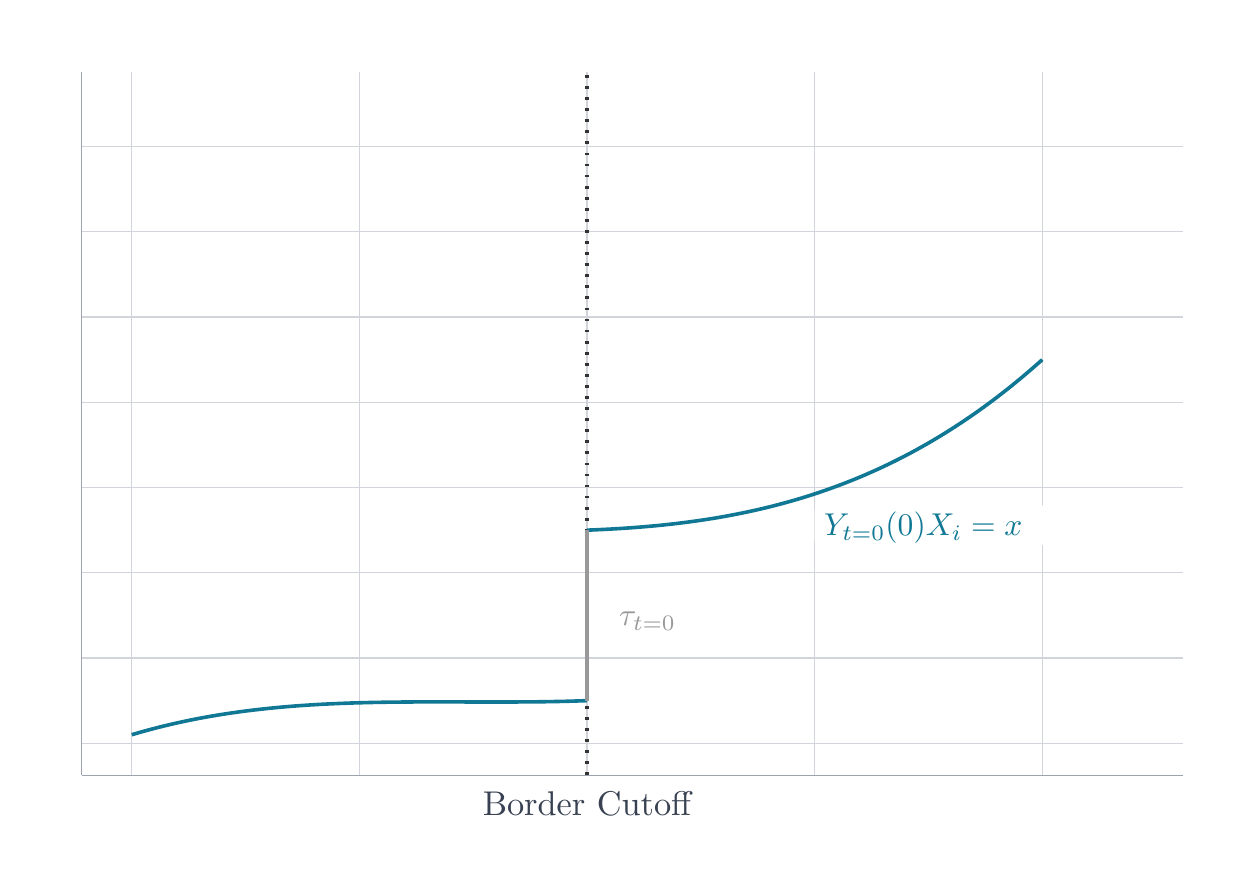
\begin{tikzpicture}[x=1pt,y=1pt]
\definecolor{fillColor}{RGB}{255,255,255}
\path[use as bounding box,fill=fillColor] (0,0) rectangle (433.62,303.53);
\begin{scope}
\path[clip] (  0.00,  0.00) rectangle (433.62,303.53);
\definecolor{drawColor}{RGB}{255,255,255}

\path[draw=drawColor,line width= 0.7pt,line join=round,line cap=round,fill=fillColor] ( -0.00,  0.00) rectangle (433.62,303.53);
\end{scope}
\begin{scope}
\path[clip] ( 19.50, 33.40) rectangle (417.62,287.53);
\definecolor{drawColor}{RGB}{255,255,255}
\definecolor{fillColor}{RGB}{255,255,255}

\path[draw=drawColor,line width= 0.7pt,line join=round,line cap=round,fill=fillColor] ( 19.50, 33.40) rectangle (417.62,287.53);
\definecolor{drawColor}{RGB}{209,213,219}

\path[draw=drawColor,line width= 0.4pt,line join=round] ( 19.50, 75.75) --
	(417.62, 75.75);

\path[draw=drawColor,line width= 0.4pt,line join=round] ( 19.50,137.36) --
	(417.62,137.36);

\path[draw=drawColor,line width= 0.4pt,line join=round] ( 19.50,198.97) --
	(417.62,198.97);

\path[draw=drawColor,line width= 0.4pt,line join=round] ( 19.50,260.58) --
	(417.62,260.58);

\path[draw=drawColor,line width= 0.4pt,line join=round] (119.85, 33.40) --
	(119.85,287.53);

\path[draw=drawColor,line width= 0.4pt,line join=round] (284.36, 33.40) --
	(284.36,287.53);

\path[draw=drawColor,line width= 0.4pt,line join=round] ( 19.50, 44.95) --
	(417.62, 44.95);

\path[draw=drawColor,line width= 0.4pt,line join=round] ( 19.50,106.56) --
	(417.62,106.56);

\path[draw=drawColor,line width= 0.4pt,line join=round] ( 19.50,168.17) --
	(417.62,168.17);

\path[draw=drawColor,line width= 0.4pt,line join=round] ( 19.50,229.78) --
	(417.62,229.78);

\path[draw=drawColor,line width= 0.4pt,line join=round] ( 37.60, 33.40) --
	( 37.60,287.53);

\path[draw=drawColor,line width= 0.4pt,line join=round] (202.11, 33.40) --
	(202.11,287.53);

\path[draw=drawColor,line width= 0.4pt,line join=round] (366.62, 33.40) --
	(366.62,287.53);
\definecolor{drawColor}{gray}{0.20}

\path[draw=drawColor,line width= 1.1pt,dash pattern=on 1pt off 3pt ,line join=round] (202.11, 33.40) -- (202.11,287.53);
\definecolor{drawColor}{RGB}{16,120,149}

\path[draw=drawColor,line width= 1.3pt,line join=round] ( 37.60, 48.03) --
	( 39.24, 48.51) --
	( 40.89, 48.99) --
	( 42.53, 49.45) --
	( 44.18, 49.89) --
	( 45.82, 50.33) --
	( 47.47, 50.75) --
	( 49.11, 51.16) --
	( 50.76, 51.55) --
	( 52.40, 51.94) --
	( 54.05, 52.31) --
	( 55.69, 52.67) --
	( 57.34, 53.02) --
	( 58.98, 53.36) --
	( 60.63, 53.69) --
	( 62.27, 54.00) --
	( 63.92, 54.31) --
	( 65.56, 54.60) --
	( 67.21, 54.88) --
	( 68.85, 55.16) --
	( 70.50, 55.42) --
	( 72.14, 55.68) --
	( 73.79, 55.92) --
	( 75.43, 56.15) --
	( 77.08, 56.38) --
	( 78.72, 56.60) --
	( 80.37, 56.80) --
	( 82.01, 57.00) --
	( 83.66, 57.19) --
	( 85.30, 57.37) --
	( 86.95, 57.55) --
	( 88.60, 57.71) --
	( 90.24, 57.87) --
	( 91.89, 58.02) --
	( 93.53, 58.16) --
	( 95.18, 58.30) --
	( 96.82, 58.43) --
	( 98.47, 58.55) --
	(100.11, 58.66) --
	(101.76, 58.77) --
	(103.40, 58.87) --
	(105.05, 58.97) --
	(106.69, 59.06) --
	(108.34, 59.14) --
	(109.98, 59.22) --
	(111.63, 59.29) --
	(113.27, 59.36) --
	(114.92, 59.42) --
	(116.56, 59.48) --
	(118.21, 59.53) --
	(119.85, 59.58) --
	(121.50, 59.62) --
	(123.14, 59.66) --
	(124.79, 59.70) --
	(126.43, 59.73) --
	(128.08, 59.76) --
	(129.72, 59.79) --
	(131.37, 59.81) --
	(133.01, 59.83) --
	(134.66, 59.84) --
	(136.30, 59.86) --
	(137.95, 59.87) --
	(139.59, 59.88) --
	(141.24, 59.88) --
	(142.88, 59.89) --
	(144.53, 59.89) --
	(146.17, 59.89) --
	(147.82, 59.89) --
	(149.46, 59.89) --
	(151.11, 59.89) --
	(152.76, 59.89) --
	(154.40, 59.89) --
	(156.05, 59.88) --
	(157.69, 59.88) --
	(159.34, 59.87) --
	(160.98, 59.87) --
	(162.63, 59.87) --
	(164.27, 59.86) --
	(165.92, 59.86) --
	(167.56, 59.86) --
	(169.21, 59.86) --
	(170.85, 59.86) --
	(172.50, 59.86) --
	(174.14, 59.86) --
	(175.79, 59.87) --
	(177.43, 59.88) --
	(179.08, 59.89) --
	(180.72, 59.90) --
	(182.37, 59.91) --
	(184.01, 59.93) --
	(185.66, 59.95) --
	(187.30, 59.97) --
	(188.95, 60.00) --
	(190.59, 60.03) --
	(192.24, 60.06) --
	(193.88, 60.10) --
	(195.53, 60.14) --
	(197.17, 60.19) --
	(198.82, 60.24) --
	(200.46, 60.29) --
	(202.11, 60.35);

\path[draw=drawColor,line width= 1.3pt,line join=round] (202.13,121.96) --
	(203.77,122.02) --
	(205.42,122.09) --
	(207.06,122.17) --
	(208.71,122.25) --
	(210.35,122.33) --
	(211.99,122.43) --
	(213.64,122.52) --
	(215.28,122.63) --
	(216.93,122.74) --
	(218.57,122.85) --
	(220.22,122.98) --
	(221.86,123.11) --
	(223.51,123.25) --
	(225.15,123.39) --
	(226.80,123.54) --
	(228.44,123.70) --
	(230.09,123.87) --
	(231.73,124.05) --
	(233.38,124.23) --
	(235.02,124.43) --
	(236.67,124.63) --
	(238.31,124.84) --
	(239.96,125.06) --
	(241.60,125.29) --
	(243.25,125.52) --
	(244.89,125.77) --
	(246.54,126.03) --
	(248.18,126.29) --
	(249.83,126.57) --
	(251.47,126.86) --
	(253.12,127.16) --
	(254.76,127.47) --
	(256.41,127.79) --
	(258.05,128.12) --
	(259.70,128.46) --
	(261.34,128.81) --
	(262.99,129.18) --
	(264.63,129.55) --
	(266.28,129.94) --
	(267.92,130.34) --
	(269.57,130.75) --
	(271.21,131.18) --
	(272.86,131.62) --
	(274.50,132.07) --
	(276.15,132.53) --
	(277.79,133.01) --
	(279.44,133.50) --
	(281.08,134.00) --
	(282.73,134.52) --
	(284.37,135.05) --
	(286.02,135.60) --
	(287.66,136.16) --
	(289.31,136.74) --
	(290.95,137.33) --
	(292.60,137.93) --
	(294.24,138.55) --
	(295.89,139.19) --
	(297.53,139.84) --
	(299.18,140.50) --
	(300.82,141.18) --
	(302.47,141.88) --
	(304.11,142.60) --
	(305.76,143.33) --
	(307.40,144.07) --
	(309.05,144.84) --
	(310.69,145.62) --
	(312.34,146.42) --
	(313.98,147.23) --
	(315.63,148.07) --
	(317.27,148.92) --
	(318.92,149.78) --
	(320.56,150.67) --
	(322.21,151.58) --
	(323.85,152.50) --
	(325.50,153.44) --
	(327.14,154.40) --
	(328.79,155.38) --
	(330.43,156.38) --
	(332.08,157.40) --
	(333.72,158.43) --
	(335.37,159.49) --
	(337.01,160.57) --
	(338.66,161.67) --
	(340.30,162.78) --
	(341.95,163.92) --
	(343.59,165.08) --
	(345.24,166.26) --
	(346.88,167.46) --
	(348.53,168.68) --
	(350.17,169.92) --
	(351.82,171.19) --
	(353.46,172.47) --
	(355.11,173.78) --
	(356.75,175.11) --
	(358.40,176.47) --
	(360.04,177.84) --
	(361.69,179.24) --
	(363.33,180.66) --
	(364.98,182.10) --
	(366.62,183.57);

\path[fill=fillColor] (286.42,116.57) --
	(385.39,116.57) --
	(385.31,116.57) --
	(385.64,116.58) --
	(385.96,116.65) --
	(386.27,116.77) --
	(386.56,116.93) --
	(386.81,117.14) --
	(387.03,117.39) --
	(387.21,117.67) --
	(387.34,117.97) --
	(387.42,118.30) --
	(387.45,118.63) --
	(387.45,118.63) --
	(387.45,128.83) --
	(387.45,128.83) --
	(387.42,129.16) --
	(387.34,129.48) --
	(387.21,129.79) --
	(387.03,130.07) --
	(386.81,130.31) --
	(386.56,130.52) --
	(386.27,130.69) --
	(385.96,130.81) --
	(385.64,130.87) --
	(385.39,130.89) --
	(286.42,130.89) --
	(286.67,130.87) --
	(286.34,130.89) --
	(286.01,130.85) --
	(285.69,130.75) --
	(285.39,130.61) --
	(285.12,130.42) --
	(284.88,130.20) --
	(284.68,129.93) --
	(284.53,129.64) --
	(284.42,129.32) --
	(284.37,129.00) --
	(284.36,128.83) --
	(284.36,118.63) --
	(284.37,118.79) --
	(284.37,118.46) --
	(284.42,118.13) --
	(284.53,117.82) --
	(284.68,117.53) --
	(284.88,117.26) --
	(285.12,117.03) --
	(285.39,116.84) --
	(285.69,116.70) --
	(286.01,116.61) --
	(286.34,116.57) --
	cycle;
\end{scope}
\begin{scope}
\path[clip] ( 19.50, 33.40) rectangle (417.62,287.53);
\definecolor{drawColor}{RGB}{16,120,149}

\node[text=drawColor,anchor=base west,inner sep=0pt, outer sep=0pt, scale=  1.14] at (287.79,120.00) {$\expec{Y_{t=0}(0)}{X_i = x}$};
\end{scope}
\begin{scope}
\path[clip] ( 19.50, 33.40) rectangle (417.62,287.53);
\definecolor{fillColor}{RGB}{255,255,255}

\path[fill=fillColor] (212.39, 84.00) --
	(235.64, 84.00) --
	(235.55, 84.00) --
	(235.88, 84.01) --
	(236.21, 84.08) --
	(236.52, 84.19) --
	(236.80, 84.36) --
	(237.06, 84.57) --
	(237.28, 84.82) --
	(237.46, 85.10) --
	(237.59, 85.40) --
	(237.67, 85.72) --
	(237.69, 86.05) --
	(237.69, 86.05) --
	(237.69, 96.26) --
	(237.69, 96.26) --
	(237.67, 96.59) --
	(237.59, 96.91) --
	(237.46, 97.21) --
	(237.28, 97.49) --
	(237.06, 97.74) --
	(236.80, 97.95) --
	(236.52, 98.12) --
	(236.21, 98.23) --
	(235.88, 98.30) --
	(235.64, 98.31) --
	(212.39, 98.31) --
	(212.64, 98.30) --
	(212.31, 98.31) --
	(211.98, 98.27) --
	(211.66, 98.18) --
	(211.36, 98.04) --
	(211.09, 97.85) --
	(210.85, 97.62) --
	(210.65, 97.36) --
	(210.50, 97.06) --
	(210.39, 96.75) --
	(210.34, 96.42) --
	(210.33, 96.26) --
	(210.33, 86.05) --
	(210.34, 86.22) --
	(210.34, 85.89) --
	(210.39, 85.56) --
	(210.50, 85.25) --
	(210.65, 84.95) --
	(210.85, 84.69) --
	(211.09, 84.46) --
	(211.36, 84.27) --
	(211.66, 84.13) --
	(211.98, 84.04) --
	(212.31, 84.00) --
	cycle;
\end{scope}
\begin{scope}
\path[clip] ( 19.50, 33.40) rectangle (417.62,287.53);
\definecolor{drawColor}{gray}{0.60}

\node[text=drawColor,anchor=base west,inner sep=0pt, outer sep=0pt, scale=  1.14] at (213.76, 87.42) {$\tau_{t=0}$};
\end{scope}
\begin{scope}
\path[clip] ( 19.50, 33.40) rectangle (417.62,287.53);
\definecolor{drawColor}{gray}{0.60}

\path[draw=drawColor,line width= 1.1pt,line join=round] (202.11, 60.35) -- (202.11,121.96);
\end{scope}
\begin{scope}
\path[clip] (  0.00,  0.00) rectangle (433.62,303.53);
\definecolor{drawColor}{RGB}{156,163,175}

\path[draw=drawColor,line width= 0.3pt,line join=round] ( 19.50, 33.40) --
	( 19.50,287.53);
\end{scope}
\begin{scope}
\path[clip] (  0.00,  0.00) rectangle (433.62,303.53);
\definecolor{drawColor}{RGB}{156,163,175}

\path[draw=drawColor,line width= 0.3pt,line join=round] ( 19.50, 33.40) --
	(417.62, 33.40);
\end{scope}
\begin{scope}
\path[clip] (  0.00,  0.00) rectangle (433.62,303.53);
\definecolor{drawColor}{RGB}{55,65,81}

\node[text=drawColor,anchor=base,inner sep=0pt, outer sep=0pt, scale=  1.24] at ( 37.60, 18.94) { };

\node[text=drawColor,anchor=base,inner sep=0pt, outer sep=0pt, scale=  1.24] at (202.11, 18.94) {Border Cutoff};

\node[text=drawColor,anchor=base,inner sep=0pt, outer sep=0pt, scale=  1.24] at (366.62, 18.94) { };
\end{scope}
\end{tikzpicture}
